% Options for packages loaded elsewhere
% Options for packages loaded elsewhere
\PassOptionsToPackage{unicode,linktoc=all}{hyperref}
\PassOptionsToPackage{hyphens}{url}
\PassOptionsToPackage{dvipsnames,svgnames,x11names}{xcolor}
%
\documentclass[
  letterpaper,
  DIV=11,
  numbers=noendperiod]{scrreprt}
\usepackage{xcolor}
\usepackage[top=30mm,left=20mm,heightrounded]{geometry}
\usepackage{amsmath,amssymb}
\setcounter{secnumdepth}{5}
\usepackage{iftex}
\ifPDFTeX
  \usepackage[T1]{fontenc}
  \usepackage[utf8]{inputenc}
  \usepackage{textcomp} % provide euro and other symbols
\else % if luatex or xetex
  \usepackage{unicode-math} % this also loads fontspec
  \defaultfontfeatures{Scale=MatchLowercase}
  \defaultfontfeatures[\rmfamily]{Ligatures=TeX,Scale=1}
\fi
\usepackage{lmodern}
\ifPDFTeX\else
  % xetex/luatex font selection
  \setmainfont[]{Calibri}
\fi
% Use upquote if available, for straight quotes in verbatim environments
\IfFileExists{upquote.sty}{\usepackage{upquote}}{}
\IfFileExists{microtype.sty}{% use microtype if available
  \usepackage[]{microtype}
  \UseMicrotypeSet[protrusion]{basicmath} % disable protrusion for tt fonts
}{}
\makeatletter
\@ifundefined{KOMAClassName}{% if non-KOMA class
  \IfFileExists{parskip.sty}{%
    \usepackage{parskip}
  }{% else
    \setlength{\parindent}{0pt}
    \setlength{\parskip}{6pt plus 2pt minus 1pt}}
}{% if KOMA class
  \KOMAoptions{parskip=half}}
\makeatother
% Make \paragraph and \subparagraph free-standing
\makeatletter
\ifx\paragraph\undefined\else
  \let\oldparagraph\paragraph
  \renewcommand{\paragraph}{
    \@ifstar
      \xxxParagraphStar
      \xxxParagraphNoStar
  }
  \newcommand{\xxxParagraphStar}[1]{\oldparagraph*{#1}\mbox{}}
  \newcommand{\xxxParagraphNoStar}[1]{\oldparagraph{#1}\mbox{}}
\fi
\ifx\subparagraph\undefined\else
  \let\oldsubparagraph\subparagraph
  \renewcommand{\subparagraph}{
    \@ifstar
      \xxxSubParagraphStar
      \xxxSubParagraphNoStar
  }
  \newcommand{\xxxSubParagraphStar}[1]{\oldsubparagraph*{#1}\mbox{}}
  \newcommand{\xxxSubParagraphNoStar}[1]{\oldsubparagraph{#1}\mbox{}}
\fi
\makeatother


\usepackage{longtable,booktabs,array}
\usepackage{calc} % for calculating minipage widths
% Correct order of tables after \paragraph or \subparagraph
\usepackage{etoolbox}
\makeatletter
\patchcmd\longtable{\par}{\if@noskipsec\mbox{}\fi\par}{}{}
\makeatother
% Allow footnotes in longtable head/foot
\IfFileExists{footnotehyper.sty}{\usepackage{footnotehyper}}{\usepackage{footnote}}
\makesavenoteenv{longtable}
\usepackage{graphicx}
\makeatletter
\newsavebox\pandoc@box
\newcommand*\pandocbounded[1]{% scales image to fit in text height/width
  \sbox\pandoc@box{#1}%
  \Gscale@div\@tempa{\textheight}{\dimexpr\ht\pandoc@box+\dp\pandoc@box\relax}%
  \Gscale@div\@tempb{\linewidth}{\wd\pandoc@box}%
  \ifdim\@tempb\p@<\@tempa\p@\let\@tempa\@tempb\fi% select the smaller of both
  \ifdim\@tempa\p@<\p@\scalebox{\@tempa}{\usebox\pandoc@box}%
  \else\usebox{\pandoc@box}%
  \fi%
}
% Set default figure placement to htbp
\def\fps@figure{htbp}
\makeatother





\setlength{\emergencystretch}{3em} % prevent overfull lines

\providecommand{\tightlist}{%
  \setlength{\itemsep}{0pt}\setlength{\parskip}{0pt}}



 


\KOMAoption{captions}{tableheading}
\makeatletter
\@ifpackageloaded{tcolorbox}{}{\usepackage[skins,breakable]{tcolorbox}}
\@ifpackageloaded{fontawesome5}{}{\usepackage{fontawesome5}}
\definecolor{quarto-callout-color}{HTML}{909090}
\definecolor{quarto-callout-note-color}{HTML}{0758E5}
\definecolor{quarto-callout-important-color}{HTML}{CC1914}
\definecolor{quarto-callout-warning-color}{HTML}{EB9113}
\definecolor{quarto-callout-tip-color}{HTML}{00A047}
\definecolor{quarto-callout-caution-color}{HTML}{FC5300}
\definecolor{quarto-callout-color-frame}{HTML}{acacac}
\definecolor{quarto-callout-note-color-frame}{HTML}{4582ec}
\definecolor{quarto-callout-important-color-frame}{HTML}{d9534f}
\definecolor{quarto-callout-warning-color-frame}{HTML}{f0ad4e}
\definecolor{quarto-callout-tip-color-frame}{HTML}{02b875}
\definecolor{quarto-callout-caution-color-frame}{HTML}{fd7e14}
\makeatother
\makeatletter
\@ifpackageloaded{caption}{}{\usepackage{caption}}
\AtBeginDocument{%
\ifdefined\contentsname
  \renewcommand*\contentsname{Table of contents}
\else
  \newcommand\contentsname{Table of contents}
\fi
\ifdefined\listfigurename
  \renewcommand*\listfigurename{List of Figures}
\else
  \newcommand\listfigurename{List of Figures}
\fi
\ifdefined\listtablename
  \renewcommand*\listtablename{List of Tables}
\else
  \newcommand\listtablename{List of Tables}
\fi
\ifdefined\figurename
  \renewcommand*\figurename{Figure}
\else
  \newcommand\figurename{Figure}
\fi
\ifdefined\tablename
  \renewcommand*\tablename{Table}
\else
  \newcommand\tablename{Table}
\fi
}
\@ifpackageloaded{float}{}{\usepackage{float}}
\floatstyle{ruled}
\@ifundefined{c@chapter}{\newfloat{codelisting}{h}{lop}}{\newfloat{codelisting}{h}{lop}[chapter]}
\floatname{codelisting}{Listing}
\newcommand*\listoflistings{\listof{codelisting}{List of Listings}}
\makeatother
\makeatletter
\makeatother
\makeatletter
\@ifpackageloaded{caption}{}{\usepackage{caption}}
\@ifpackageloaded{subcaption}{}{\usepackage{subcaption}}
\makeatother
\usepackage{bookmark}
\IfFileExists{xurl.sty}{\usepackage{xurl}}{} % add URL line breaks if available
\urlstyle{same}
\hypersetup{
  pdftitle={IC Design of a Universal Biquad Filter},
  pdfauthor={Aditya Ranjan Shandilya; Merlin Anitha Athisayaraj},
  colorlinks=true,
  linkcolor={blue},
  filecolor={Maroon},
  citecolor={Blue},
  urlcolor={Blue},
  pdfcreator={LaTeX via pandoc}}


\title{IC Design of a Universal Biquad Filter}
\author{Aditya Ranjan Shandilya \and Merlin Anitha Athisayaraj}
\date{2025-07-16}
\begin{document}
\maketitle
\begin{abstract}
Lorem ipsum
\end{abstract}

\renewcommand*\contentsname{Table of contents}
{
\hypersetup{linkcolor=}
\setcounter{tocdepth}{2}
\tableofcontents
}

\chapter{Introduction}\label{introduction}

As the availability of standardized integrated circuit solutions
continues to diminish, the demand for tailored, application-specific
analog and mixed-signal designs is steadily increasing
(\textbf{Dobkin2011?}). Reflecting this shift, students enrolled in the
``Concept Engineering Mixed-Technology Systems'' course, taught by
Professor Meiners at The City University of Applied Sciences, have been
tasked with designing a biquadratic filter. The goal is to create a
high-performance, application-specific solution suitable for integration
within a defined analog front-end system.

Analog signal processing remains a foundational element of modern
electronic design. Despite rapid advancements in digital
technology---characterized by nanometer-scale fabrication and
Gigahertz-level processing speeds---the real world continues to present
signals in analog form. Therefore, analog circuitry, particularly in the
front-end of many systems, plays a critical role in conditioning signals
before digitization (\textbf{kester2005data?}).

In mixed-signal systems, analog signal processing is increasingly being
paired with powerful digital post-processing techniques. This synergy
allows engineers to rely on cost-effective analog components while
compensating for their limitations through digital correction and
enhancement methods (\textbf{Baker2008?}). However, before digital
techniques can be applied, analog filtering remains essential for tasks
such as noise suppression, anti-aliasing, and band selection.
Biquadratic filters---due to their versatile frequency response
characteristics and relatively simple implementation---are widely used
in these contexts.

\section{Objective of the lab}\label{objective-of-the-lab}

To design a biquad active filter with a corner frequency (ω0) of 1 kHz
and a Q-factor of 10, and to understand its frequency characteristics.

\section{Motivation: importance of second-order (biquad)
filters}\label{motivation-importance-of-second-order-biquad-filters}

Second-order filters, also known as biquad filters, are fundamental in
constructing higher-order filters:

\begin{itemize}
\tightlist
\item
  They serve as building blocks for \(N^{\text{th}}\) order filters when
  \(N > 2\).
\item
  For odd values of \(N\), an \(N^{\text{th}}\) order filter can be
  implemented using \(\frac{N - 1}{2}\) second-order filters and one
  first-order filter.
\item
  For even values of \(N\), \(\frac{N}{2}\) second-order filters are
  required to realize an \(N^{\text{th}}\) order filter.
\end{itemize}

\chapter{Filter Design Fundamentals}\label{filter-design-fundamentals}

\section{Second order universal active
filter}\label{second-order-universal-active-filter}

\begin{figure}[H]

{\centering \pandocbounded{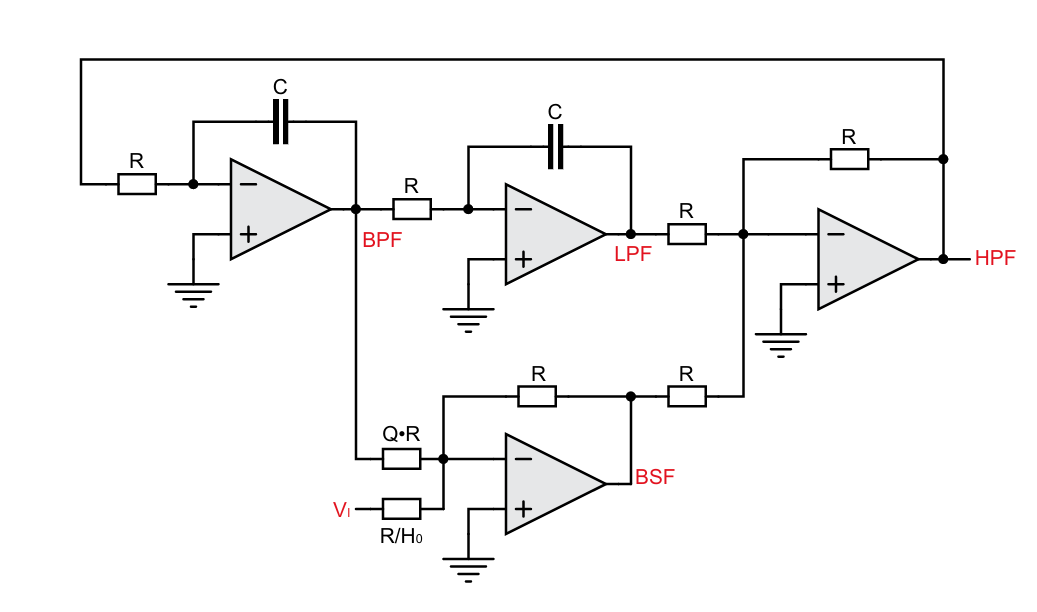
\includegraphics[keepaspectratio]{images/Second order universal active filter.png}}

}

\caption{Second order universal active filter}

\end{figure}%

The circuit diagram shows a \textbf{universal active filter} capable of
producing four different types of outputs simultaneously. It is
constructed from four operational transcundactance amplifiers - two
inverting intergrators, 2 inverting adders, resistors, and capacitors.

\begin{itemize}
\tightlist
\item
  \textbf{BPF Output}: First Integrator (top-left op-amp) processes the
  input signal.
\item
  \textbf{LPF Output}: Second Integrator (top-middle op-amp) takes the
  BPF output as its input.
\item
  \textbf{HPF Output}: Inverting Adder 1 (top-right op-amp) sums the LPF
  output, the BPF output, and the original input signal.
\item
  \textbf{BSF Output}: Inverting Adder 2 (bottom op-amp) sums the LPF
  and HPF outputs.
\end{itemize}

\section{The Inverting Adder}\label{the-inverting-adder}

An inverting adder (or summing amplifier) outputs a voltage that is the
inverted, weighted sum of its input voltages.

\subsection{Output Voltage Equation}\label{output-voltage-equation}

For an inverting adder with three inputs (\(V_a, V_b, V_c\)), input
resistors (\(R_a, R_b, R_c\)), and a feedback resistor (\(R_f\)), the
output voltage \(V_o\) is:

\[
V_o = - \left( \frac{R_f}{R_a}V_a + \frac{R_f}{R_b}V_b + \frac{R_f}{R_c}V_c \right)
\]

\section{The Inverting Integrator}\label{the-inverting-integrator}

An inverting integrator is an operational amplifier circuit that
produces an output voltage proportional to the time integral of its
input voltage, with an inverted sign. It's fundamentally an inverting
amplifier with a capacitor in the feedback path.

\subsection{Output Voltage Equation}\label{output-voltage-equation-1}

For an inverting integrator with an input voltage (\(V_i\)), an input
resistor (\(R_1\)), and a feedback capacitor (\(C_f\)), the output
voltage \(V_o\) is:

\[V_o = - \frac{1}{R_1 C_f} \int V_i \, dt + V_o(0)\]

\section{Transfer function}\label{transfer-function}

The biquadratic filter, or ``biquad,'' is a second-order filter widely
used in analog filter design. Its general transfer function is given by:
\[H(s)=\frac{a_{1}s^{2}+b_{1}s+c_{1}}{a_{2}s^{2}+b_{2}s+c_{2}}\]

The numerator coefficients can be chosen to achieve low-pass, band-pass,
or high-pass responses. For example, setting \(a_{1}=b_{1}=0\) leads to
a low-pass filter (LPF). Higher-order filters can be constructed by
cascading biquad sections.

Second-order filters can realize four types of filters, with their
transfer functions typically shown below.

Here are the transfer functions for common second-order active filters:

\begin{itemize}
\item
  \textbf{Low Pass Filter (LPF)}:
  \[\frac{V_{03}}{V_{i}}=\frac{+H_{0}}{(1+\frac{s}{\omega_{0}Q}+\frac{s^{2}}{\omega_{0}^{2}})}\]
\item
  \textbf{High Pass Filter (HPF)}:
  \[\frac{V_{01}}{V_{i}}=\frac{(H_{0}\cdot\frac{S^{2}}{G_{i}^{2}})}{(1+\frac{S}{a_{0}Q}+\frac{S^{2}}{a_{0}^{2}})}\]
\item
  \textbf{Band Pass Filter (BPF)}:
  \[\frac{V_{02}}{V_{i}}=\frac{(-H_{0}\cdot\frac{S}{Q_{0}})}{(1+\frac{S}{Q_{0}Q}+\frac{S^{2}}{Q_{0}^{2}})}\]
\item
  \textbf{Band Stop Filter (BSF)}:
  \[\frac{V_{o4}}{V_{i}}=\frac{(1+\frac{s^{2}}{Q_{o}^{2}})\cdot H_{0}}{(1+\frac{s}{Q_{o}Q}+\frac{s^{2}}{Q_{o}^{2}})}\]
\end{itemize}

\chapter{Behavioral Model Analysis using
python}\label{behavioral-model-analysis-using-python}

This sectio presents the behavioral analysis of the designed system
using Python. The analysis primarily includes the \textbf{frequency
response} (magnitude and phase response) and \textbf{transient
analysis}.

\begin{center}\rule{0.5\linewidth}{0.5pt}\end{center}

\section{1. Objective}\label{objective}

To evaluate the performance of the behavioral model through simulation
using Python, focusing on:

\begin{itemize}
\tightlist
\item
  Magnitude response
\item
  Phase response
\item
  Transient behavior
\end{itemize}

\begin{center}\rule{0.5\linewidth}{0.5pt}\end{center}

\section{2. Frequency Response
Analysis}\label{frequency-response-analysis}

\subsection{2.1 Magnitude Response}\label{magnitude-response}

The magnitude response of the system was plotted to observe how the
system amplifies or attenuates input signals across different
frequencies. The Bode magnitude plot gives a clear insight into the
bandwidth and gain characteristics.

\subsection{2.2 Phase Response}\label{phase-response}

The phase response of the system was analyzed to study the phase shift
introduced at various frequencies. This is essential for understanding
the signal integrity and phase margin.

\begin{figure}[H]

{\centering \pandocbounded{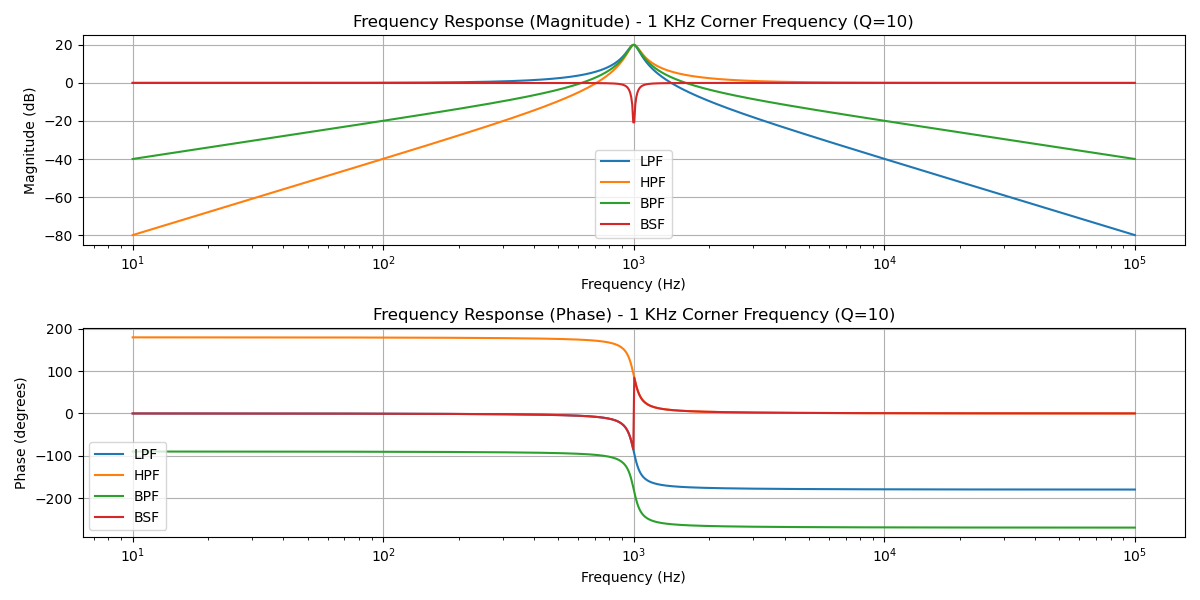
\includegraphics[keepaspectratio]{images/frequency_response_1KHz_Q10.png}}

}

\caption{Magnitude Response}

\end{figure}%

\section{3. Transient Analysis}\label{transient-analysis}

Transient analysis was performed to examine how the system responds to a
time-domain input.

\begin{figure}[H]

{\centering \pandocbounded{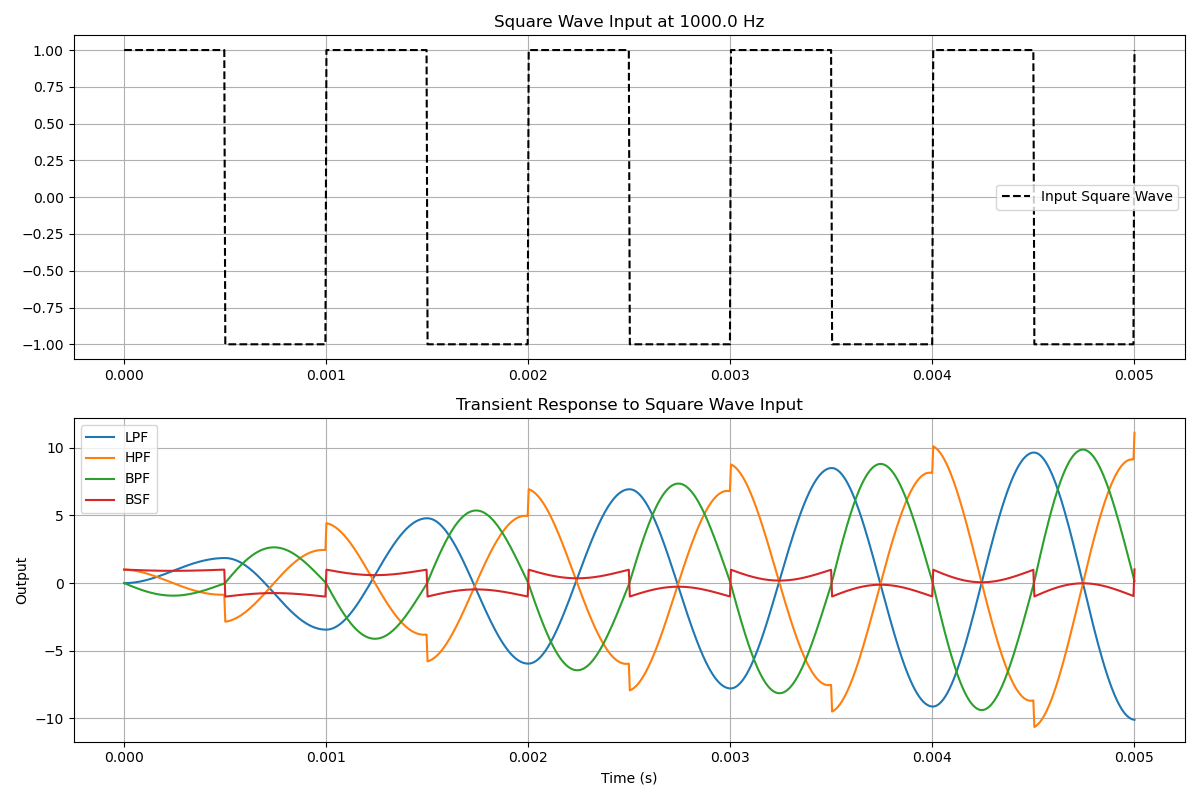
\includegraphics[keepaspectratio]{images/transient_response_1KHz_Q10.pdf}}

}

\caption{Transient Response}

\end{figure}%

\section{4. Conclusion}\label{conclusion}

The behavioral model demonstrates expected frequency and time-domain
characteristics, validating the design for further implementation. The
results align with theoretical expectations, making it suitable for the
next stages of circuit/system development.

\chapter{Circuit Design and Simulation in
Xschem}\label{circuit-design-and-simulation-in-xschem}

This section details the process of designing and simulating the
second-order biquad filter using Xschem and ngspice. Our methodology
progressed from an ideal, op-amp-based circuit to a more practical,
transistor-level implementation, allowing for a comparative analysis of
ideal and real-world performance.

\section{Ideal Circuit: Universal Active
Filter}\label{ideal-circuit-universal-active-filter}

Our initial approach was to implement a universal second-order biquad
filter based on the topology described in Experiment 4 of the Texas
Instruments ASLK Pro Manual. This architecture is valuable because it
simultaneously provides low-pass (LPF), high-pass (HPF), band-pass
(BPF), and band-stop (BSF) outputs from a single circuit.

\subsection{Circuit Topology and
Theory}\label{circuit-topology-and-theory}

The filter is based on the Tow-Thomas biquad topology, which uses two
integrators and an inverter to realize the filter transfer functions.
The general schematic is shown in Figure~\ref{fig-ideal-uni}.

\begin{figure}

\centering{

\pandocbounded{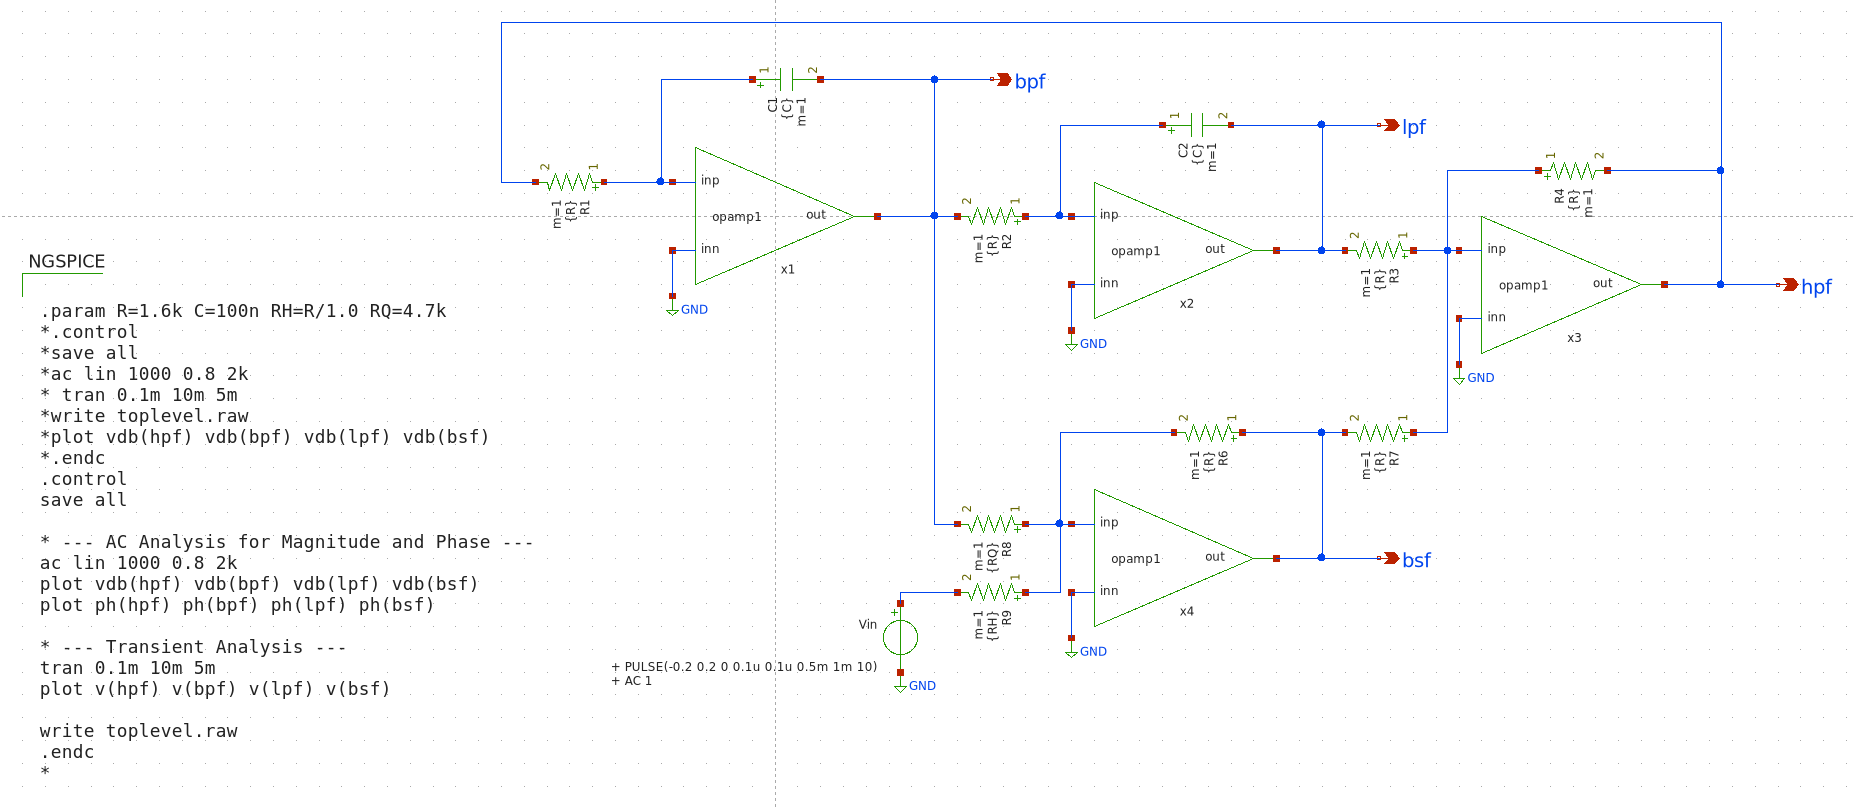
\includegraphics[keepaspectratio]{images/ideal-biquad-uni.png}}

}

\caption{\label{fig-ideal-uni}Schematic of the ideal universal
second-order active filter, based on the ASLK Pro manual.}

\end{figure}%

\subsection{Ideal Op-Amp Model and Symbol
Creation}\label{ideal-op-amp-model-and-symbol-creation}

To simulate the ideal behavior of this circuit, we first required an
ideal operational amplifier model. We used a standard single-pole op-amp
SPICE model from eCircuit Center, shown in \textbf{?@lst-opamp-subckt}.

\textbf{Implementation Note:} A common pitfall during setup is the path
configuration for custom models. Xschem initially searches for model
files in the project's home directory. We had to configure the
simulation settings to ensure Xschem could locate the
\texttt{OPAMP1.cir} file in our circuit's working directory.

\subsection{Simulation and Results}\label{simulation-and-results}

With the ideal op-amp symbol and model in place, we constructed the
schematic for the universal biquad filter. We then wrote an ngspice
script (\textbf{?@lst-ideal-uni-sim}) to perform the analysis.

\subsection{Frequency Response Analysis - Magnitude
Response}\label{frequency-response-analysis---magnitude-response}

The magnitude response of the system was plotted to observe how the
system amplifies or attenuates input signals across different
frequencies. The Bode magnitude plot gives a clear insight into the
bandwidth and gain characteristics.

\begin{figure}[H]

{\centering \pandocbounded{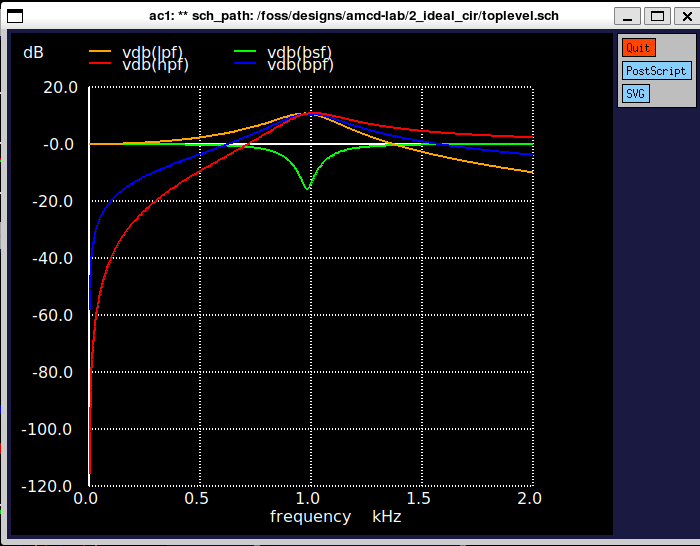
\includegraphics[keepaspectratio]{images/mag_resp.png}}

}

\caption{Magnitude Response}

\end{figure}%

\subsection{Phase Response}\label{phase-response-1}

The phase response of the system was analyzed to study the phase shift
introduced at various frequencies. This is essential for understanding
the signal integrity and phase margin.

\begin{figure}[H]

{\centering \pandocbounded{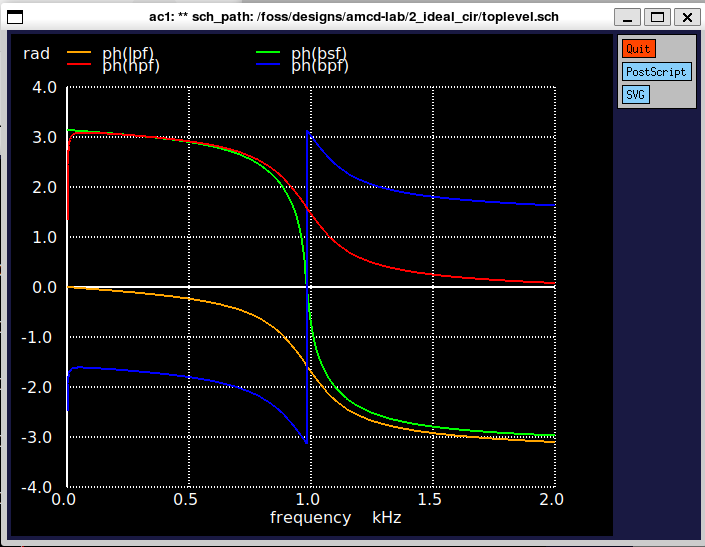
\includegraphics[keepaspectratio]{images/phase_resp.png}}

}

\caption{Phase Response}

\end{figure}%

\subsection{Transient Analysis}\label{transient-analysis-1}

Transient analysis was performed to examine how the system responds to a
time-domain input.

\begin{figure}[H]

{\centering \pandocbounded{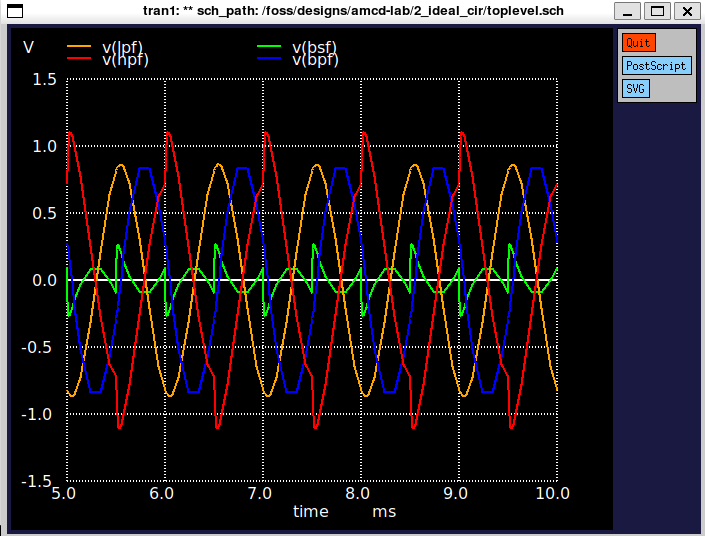
\includegraphics[keepaspectratio]{images/transient_response_ideal.png}}

}

\caption{Transient Response}

\end{figure}%

The plot clearly shows the expected behavior for each filter type,
centered around 1 kHz. The BPF peaks at the center frequency, while the
BSF shows a notch at the same point.

\section{Real Circuit: Gm-C Biquad
Filter}\label{real-circuit-gm-c-biquad-filter}

This section details the transition from an ideal circuit simulation to
a practical, transistor-level implementation. The core of this process
is replacing the ideal op-amp model with a custom-designed Operational
Transconductance Amplifier (OTA) within the IHP Microelectronics SG13G2
130nm CMOS technology.

\subsection{Initial Approach: The 5-Transistor
OTA}\label{initial-approach-the-5-transistor-ota}

Our first step towards a real circuit was to design and size a
fundamental analog building block: the 5-Transistor (5T) OTA.

\subsubsection{From an Ideal Model to a Transistor-Level
Circuit}\label{from-an-ideal-model-to-a-transistor-level-circuit}

In the initial phase of the project, we used an ideal op-amp, which is a
behavioral model in SPICE. It assumes infinite gain, infinite bandwidth,
and zero output impedance. This is useful for verifying circuit topology
and transfer functions at a conceptual level.

A real OTA, however, is built from transistors and has inherent physical
limitations: * \textbf{Finite Gain and Bandwidth}: The voltage gain is
limited by the transistor's output impedance and transconductance. *
\textbf{Power Consumption}: It draws a finite DC current from the power
supply. * \textbf{Non-linearities}: Its behavior can deviate from the
ideal linear model, especially with large input signals. *
\textbf{Noise}: The transistors introduce electronic noise into the
circuit.

Transitioning to a transistor-level OTA is therefore essential for
designing a circuit that can be physically manufactured and will perform
predictably.

\subsubsection{Anatomy of a 5T OTA}\label{anatomy-of-a-5t-ota}

The 5T OTA is a cornerstone of analog design due to its simplicity and
efficiency. It consists of a differential input pair (M1, M2), a
current-mirror active load (M3, M4), and a tail current source (M5)
which sets the amplifier's bias point.

\begin{figure}

\centering{

\pandocbounded{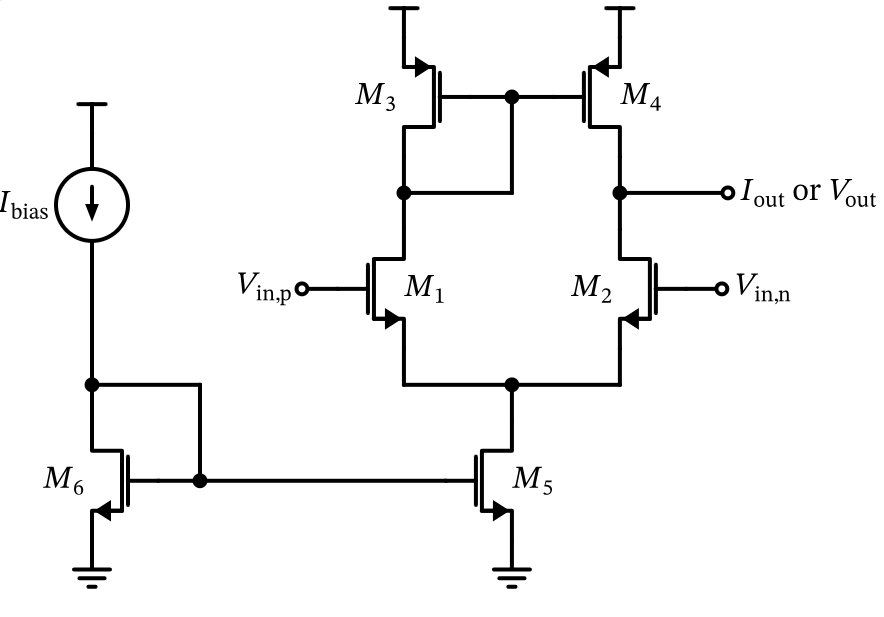
\includegraphics[keepaspectratio]{images/basic-5T-OTA.png}}

}

\caption{\label{fig-Basic-5T-OTA-Schematic}Basic 5T OTA Schematic}

\end{figure}%

In this circuit: - \textbf{M1 and M2} form the input differential pair.
They operate in the saturation region, where the drain current is
controlled by the gate-source voltage (\(V_{GS}\)). The differential
input voltage (\(V_{in,p} - V_{in,n}\)) creates a differential current
between the two branches. - \textbf{M3 and M4} form a PMOS current
mirror that acts as the active load. This configuration provides a high
output impedance, which helps achieve a higher voltage gain compared to
a simple resistive load. - \textbf{M5} is the tail current source, which
provides a constant bias current (\(I_{tail}\)) to the differential
pair. This current is mirrored from a reference current source via M6.

The transconductance (\(g_m\)) of the OTA is primarily set by the
characteristics of the input pair and its bias current.

\subsubsection{\texorpdfstring{Sizing the 5T OTA with the \texttt{gm/ID}
Methodology}{Sizing the 5T OTA with the gm/ID Methodology}}\label{sizing-the-5t-ota-with-the-gmid-methodology}

To determine the transistor dimensions (W/L), we used the modern
\texttt{gm/ID} sizing methodology. This approach utilizes
pre-characterized lookup tables from foundry data (in our case, SG13G2)
to achieve an optimal balance between performance metrics like gain,
speed, and power.

The quantitative sizing process is summarized below.

\textbf{Design Specifications \& Key Parameters}

\begin{longtable}[]{@{}
  >{\raggedright\arraybackslash}p{(\linewidth - 4\tabcolsep) * \real{0.2674}}
  >{\raggedright\arraybackslash}p{(\linewidth - 4\tabcolsep) * \real{0.2558}}
  >{\raggedright\arraybackslash}p{(\linewidth - 4\tabcolsep) * \real{0.4767}}@{}}
\toprule\noalign{}
\begin{minipage}[b]{\linewidth}\raggedright
Parameter
\end{minipage} & \begin{minipage}[b]{\linewidth}\raggedright
Value
\end{minipage} & \begin{minipage}[b]{\linewidth}\raggedright
Description
\end{minipage} \\
\midrule\noalign{}
\endhead
\bottomrule\noalign{}
\endlastfoot
Technology & SG13G2 130nm & IHP Microelectronics CMOS process \\
Load Capacitance & 50 fF & Assumed load for bandwidth calculation \\
Target Bandwidth & 10 MHz & -3dB bandwidth target for the OTA \\
Total Current Limit & 10 µA & Maximum allowed supply current \\
PMOS \texttt{gm/ID} (M3, M4) & 5 S/A & Operating point for the active
load \\
NMOS \texttt{gm/ID} (M1, M2) & 10 S/A & Operating point for the
differential pair \\
Channel Length (L) & 5 µm & Chosen for high intrinsic gain
(\texttt{gm/gds}) \\
\end{longtable}

\textbf{Quantitative Sizing Analysis}

\begin{enumerate}
\def\labelenumi{\arabic{enumi}.}
\item
  \textbf{Required Transconductance (\(g_m\))}: The target bandwidth
  (\(f_{bw}\)) for a given load (\(C_{load}\)) dictates the required
  transconductance of the input pair. We include a margin of 3x to
  account for parasitics.
  \[ g_{m1,2} = f_{bw} \times 3 \times 4\pi C_{load} = 10 \text{ MHz} \times 3 \times 4\pi \times 50 \text{ fF} \approx 18.8 \text{ µS} \]
\item
  \textbf{Bias Current Calculation}: With a target \texttt{gm/ID} of 10
  S/A for the input pair, the required drain current per transistor is:
  \[ I_{D1,2} = \frac{g_{m1,2}}{g_m/I_D} = \frac{18.8 \text{ µS}}{10 \text{ S/A}} = 1.88 \text{ µA} \]
  The total tail current is
  \(I_{tail} = 2 \times I_{D1,2} = 3.76 \text{ µA}\), which was rounded
  up to \textbf{4.0 µA}. This meets our power consumption target of
  \textless{} 10 µA.
\item
  \textbf{DC Gain (\(A_0\)) Calculation}: The DC voltage gain is the
  transconductance divided by the total output conductance
  (\(g_{ds1,2} + g_{ds3,4}\)). Using the lookup tables to find the
  intrinsic gain (\texttt{gm/gds}) for our chosen operating points and
  \texttt{L=5µm}:
  \[ A_0 = \frac{g_{m1,2}}{g_{ds1,2} + g_{ds3,4}} \Rightarrow 20 \log_{10}(A_0) \approx 34.8 \text{ dB} \]
\item
  \textbf{Transistor Widths (W)}: The final step is to find the
  transistor widths that provide the required currents for the chosen
  \texttt{gm/ID} and \texttt{L}. This is done by looking up the current
  density (\texttt{ID/W}) and calculating \(W = I_D / (I_D/W)\).
\end{enumerate}

Based on this quantitative sizing, the following schematic was created
in Xschem, representing the physical implementation of our basic 5T OTA.

\begin{figure}

\centering{

\pandocbounded{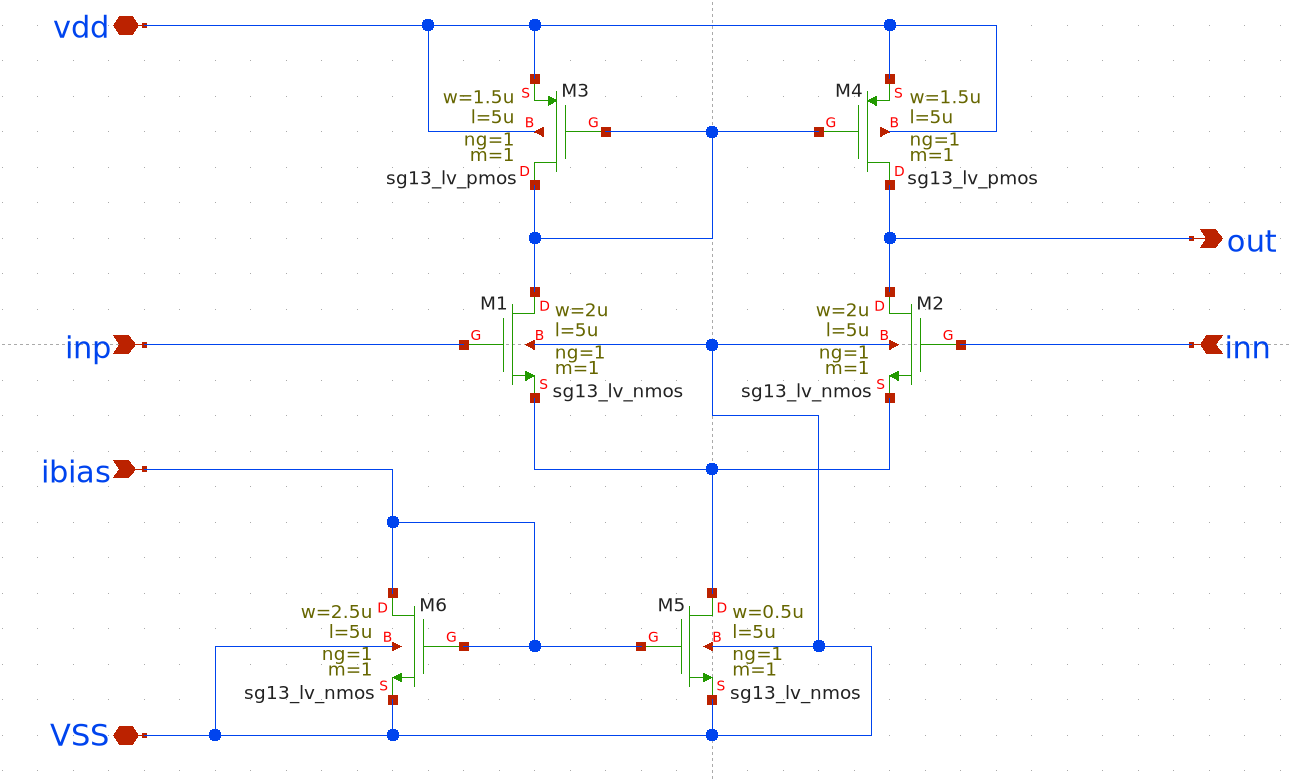
\includegraphics[keepaspectratio]{images/basic-5T-OTA-xschem.png}}

}

\caption{\label{fig-Basic-5T-OTA-Xschem}Xschem implementation of the
sized 5T OTA}

\end{figure}%

\subsection{Implementation with the Universal Biquad
Filter}\label{implementation-with-the-universal-biquad-filter}

With a basic OTA designed, we moved to implement a filter. For this, we
used an initial 5T OTA design from Professor Pretl's documentation as a
reference, primarily because it included additional biasing circuitry
for enable/disable functionality. For this implementation, a bias
current (\texttt{I\_bias}) of \textbf{20µA} was used.

The schematic below shows this specific OTA. In addition to the core 5T
structure (M1-M5), it includes transistors (M7, M8, M12, M13) controlled
by enable signals (\texttt{ena}, \texttt{d\_ena}) that can shut down the
bias currents to turn the OTA off.

\begin{figure}

\centering{

\pandocbounded{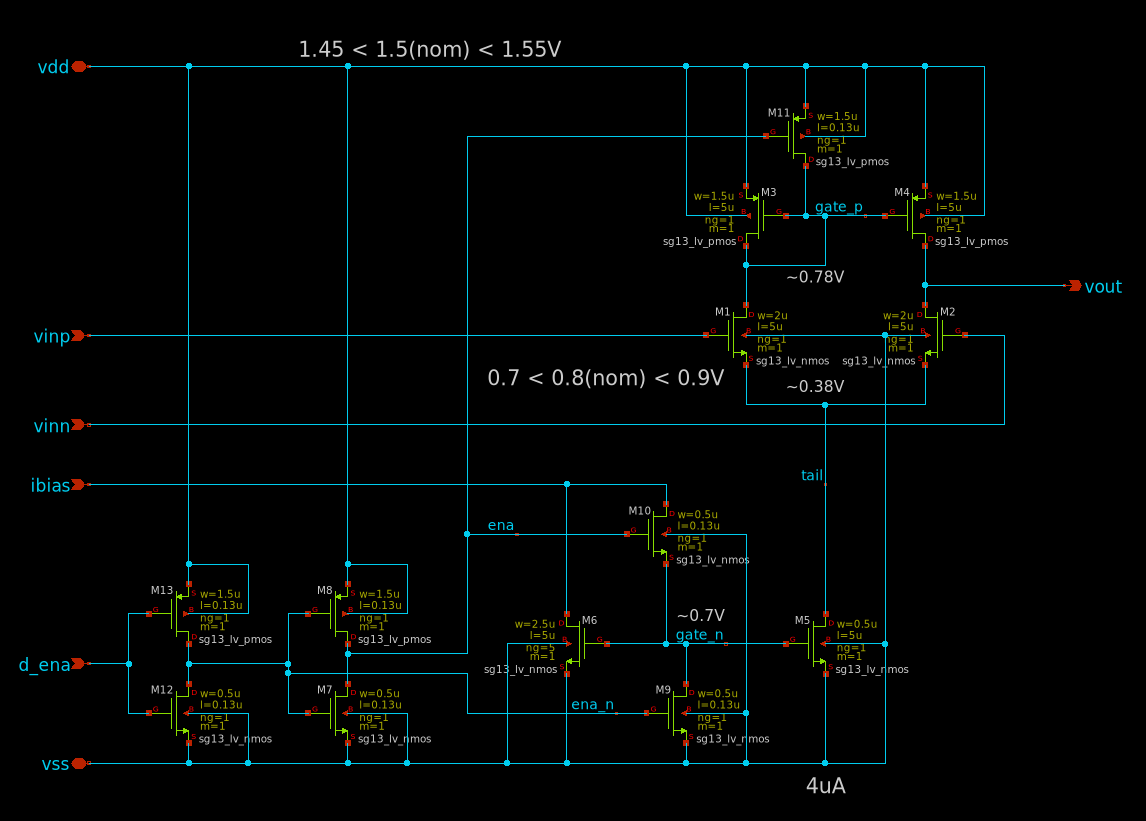
\includegraphics[keepaspectratio]{images/ota-5t-pretl.png}}

}

\caption{\label{fig-Pretl-OTA}Xschem schematic of the 5T OTA used in the
filter.}

\end{figure}%

We then replaced the ideal op-amp blocks in our universal biquad filter
with this real, transistor-level OTA. This is a critical step: while the
ideal circuit verifies the mathematical correctness of the filter
topology, the real circuit tests whether the design can function with
the physical limitations (finite gain, low drive current) of the chosen
OTA.

\begin{figure}

\centering{

\pandocbounded{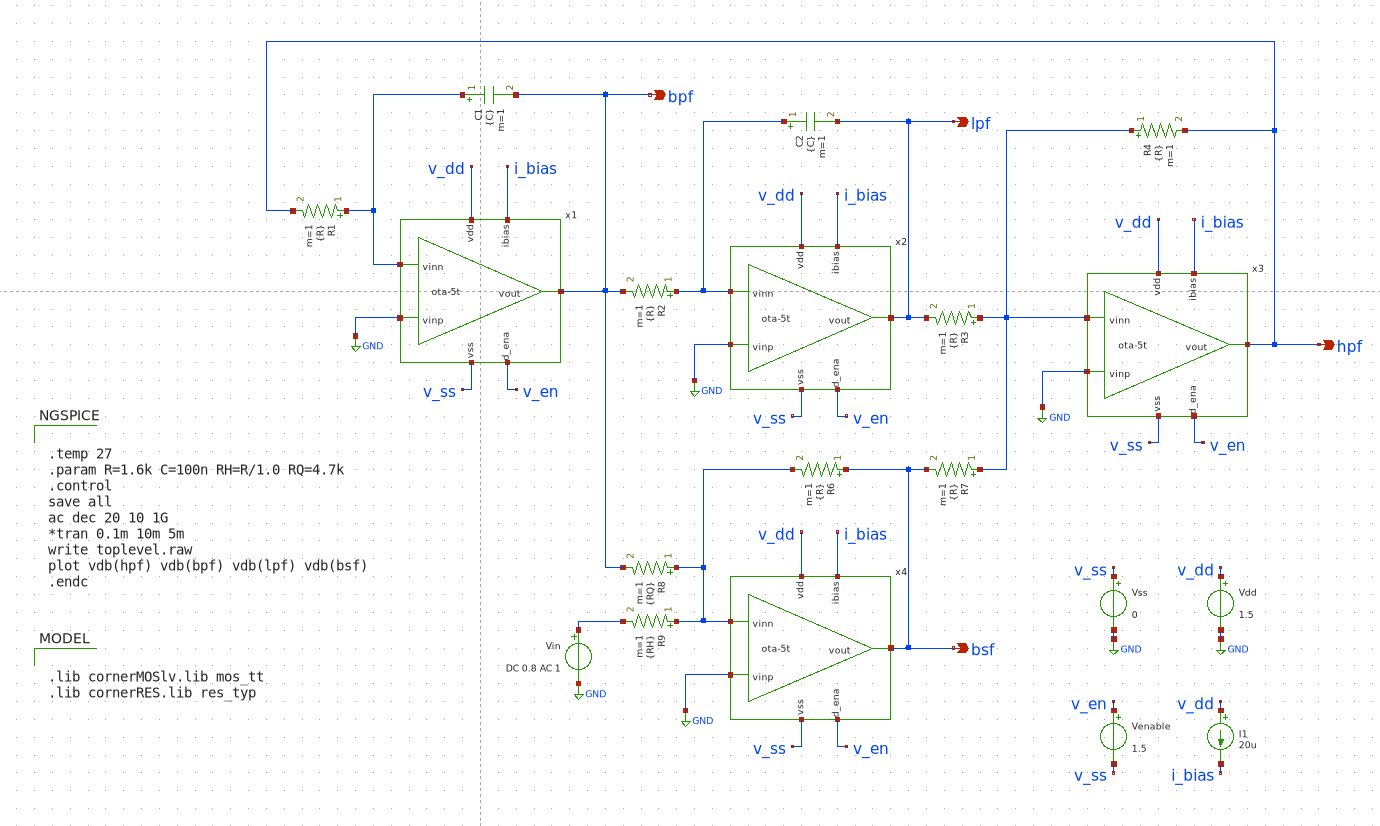
\includegraphics[keepaspectratio]{images/real-biquad-uni.png}}

}

\caption{\label{fig-Universal-Biquad}Xschem schematic of the Universal
Biquad Filter using the real 5T OTA.}

\end{figure}%

\subsubsection{Simulation and Analysis of
Failure}\label{simulation-and-analysis-of-failure}

The AC analysis of the real-circuit universal biquad produced the
following results, which represent a complete failure of the filter.

\begin{figure}

\centering{

\pandocbounded{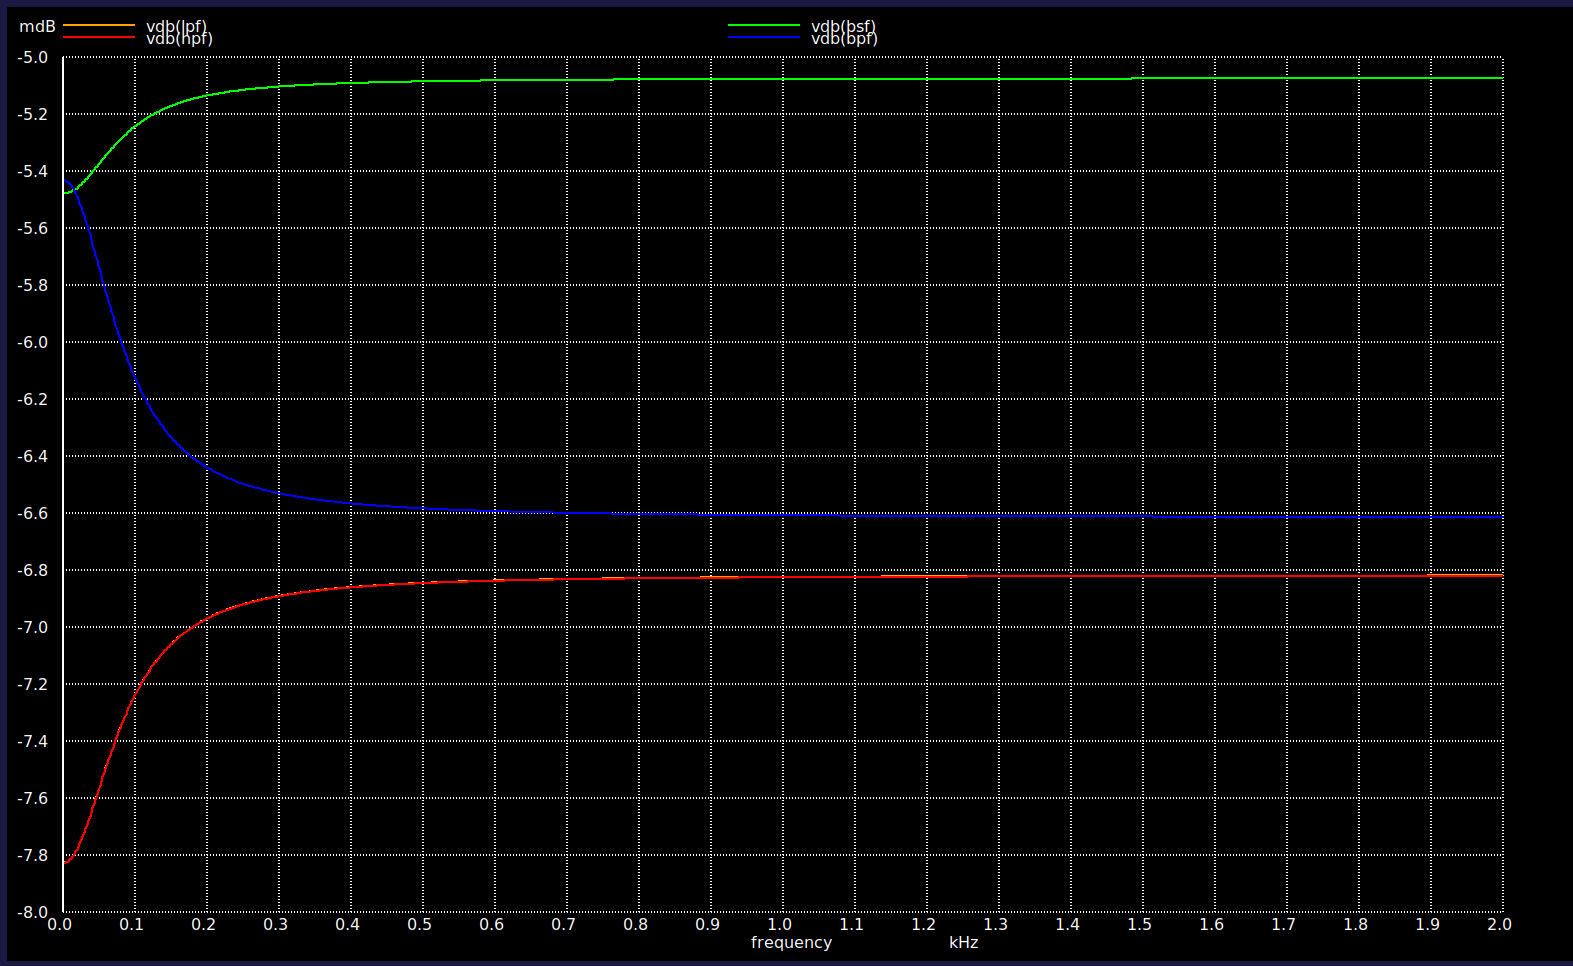
\includegraphics[keepaspectratio]{images/real-biquad-uni-output.png}}

}

\caption{\label{fig-Universal-Biquad-Output}AC simulation results for
the Universal Biquad Filter.}

\end{figure}%

The results unequivocally show that the circuit is not performing any
filtering. This failure is a direct consequence of the OTA's poor
performance, particularly its low DC gain (\textasciitilde35 dB) and
insufficient drive current, which are unable to make the integrator
loops in the biquad operate correctly.

\subsection{Design Challenges and
Pivot}\label{design-challenges-and-pivot}

The unsuccessful simulation of the universal biquad filter highlighted
critical flaws in our initial approach:

\begin{enumerate}
\def\labelenumi{\arabic{enumi}.}
\tightlist
\item
  \textbf{Topology Unsuitability}: The universal biquad topology, while
  versatile in theory, proved overly complex and sensitive for a
  practical IC implementation with a simple OTA.
\item
  \textbf{OTA Performance Limitations}: The quantitative analysis and
  simulation results confirmed that the 5T OTA was the primary
  bottleneck. The DC gain was insufficient for a high-Q filter, and the
  drive current was too low.
\end{enumerate}

These findings necessitated a complete redesign of both the filter
topology and the core amplifier.

\subsection{A New Direction: Baker's Gm-C Biquad
Filter}\label{a-new-direction-bakers-gm-c-biquad-filter}

We pivoted to a more robust design by referencing R. Jacob Baker's
\emph{CMOS Mixed-Signal Circuit Design}. We selected a \textbf{Gm-C
biquad filter} topology and set out to design a high-performance, fully
differential OTA to drive it.

\subsubsection{High-Performance Fully Differential OTA: Conceptual
Architecture}\label{high-performance-fully-differential-ota-conceptual-architecture}

The chosen architecture is a fully differential OTA designed to convert
a differential input voltage into a differential output current. It is
composed of three main functional blocks.

\begin{figure}

\centering{

\pandocbounded{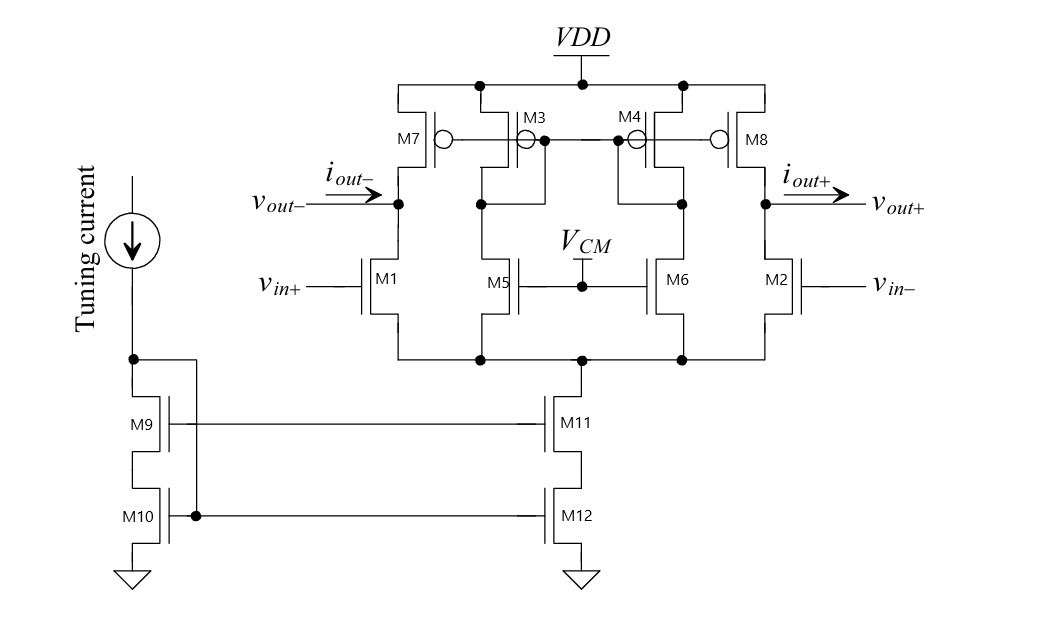
\includegraphics[keepaspectratio]{images/ota-baker-book.jpg}}

}

\caption{\label{fig-Baker-OTA}Conceptual schematic of the fully
differential OTA from Baker.}

\end{figure}%

\begin{itemize}
\item
  \textbf{Main Amplifier Stage}: The core is a single-stage differential
  amplifier. Transistors \textbf{M1} and \textbf{M2} form the NMOS input
  differential pair. \textbf{M7} and \textbf{M8} are PMOS transistors
  acting as an active load, sourcing current into the output nodes
  (\texttt{vout+}, \texttt{vout-}) and providing high output resistance
  for gain. \textbf{M11} is a tail current source that sets the DC bias
  for the input pair.
\item
  \textbf{Biasing Circuit}: The section on the left, with the
  \textbf{Tuning Current} source and diode-connected transistors
  \textbf{M9} and \textbf{M10}, is the master biasing circuit. The
  external tuning current establishes stable gate-to-source voltages
  that are then used to bias the gates of \textbf{M11} and \textbf{M12}
  via current mirroring.
\item
  \textbf{Common-Mode Feedback (CMFB) Circuit}: In a fully differential
  amplifier, the DC level of the outputs must be precisely defined. The
  CMFB circuit (\textbf{M3-M6}, \textbf{M12}) senses the common-mode
  voltage of the outputs, compares it to a reference voltage
  (\textbf{VCM}), and creates a negative feedback loop by adjusting the
  gate voltage of the active load transistors (\textbf{M7, M8}). This
  locks the output common-mode voltage at a stable, desired level.
\end{itemize}

\subsubsection{Sizing the High-Performance
OTA}\label{sizing-the-high-performance-ota}

We adapted the \texttt{gm/ID} methodology to size this more complex OTA.
The design goals for this amplifier were significantly more ambitious
than for the initial 5T OTA, targeting higher gain and drive current
suitable for a high-performance filter.

\textbf{New Design Specifications}

\begin{longtable}[]{@{}
  >{\raggedright\arraybackslash}p{(\linewidth - 4\tabcolsep) * \real{0.2840}}
  >{\raggedright\arraybackslash}p{(\linewidth - 4\tabcolsep) * \real{0.2716}}
  >{\raggedright\arraybackslash}p{(\linewidth - 4\tabcolsep) * \real{0.4444}}@{}}
\toprule\noalign{}
\begin{minipage}[b]{\linewidth}\raggedright
Parameter
\end{minipage} & \begin{minipage}[b]{\linewidth}\raggedright
Value
\end{minipage} & \begin{minipage}[b]{\linewidth}\raggedright
Comparison with 5T OTA
\end{minipage} \\
\midrule\noalign{}
\endhead
\bottomrule\noalign{}
\endlastfoot
Target DC Gain & 60 dB & Much higher than the 35 dB achieved \\
Input Bias Current & 100 µA & A 5x increase over the 20µA used \\
\texttt{gm/ID} (Input Pair) & 18 S/A & Higher efficiency (weaker
inversion) \\
Channel Length (L) & 0.5 µm & Shorter, for higher speed \\
\end{longtable}

\textbf{Quantitative Sizing Analysis}

The sizing began with the bandwidth requirement, which sets the needed
transconductance.
\[ g_{m1,2} = f_{bw} \times 2\pi C_{load} \times (\text{Safety Factor}) = 10\text{e}6 \times 2\pi \times 50\text{e-15} \times 3 \approx 10 \text{ µS} \]
From this, the bias currents for the differential pair and the tail
current were calculated:
\[ I_{D1,2} = \frac{g_{m1,2}}{g_m/I_D} = \frac{10 \text{ µS}}{18 \text{ S/A}} \approx 0.52 \text{ µA} \]
\[ I_{tail} = 2 \times I_{D1,2} \approx 1.05 \text{ µA} \]

The crucial step was the DC gain calculation. The gain is set by the
input transconductance and the total output resistance
(\(r_{o,total} = r_{o,nmos} || r_{o,pmos}\)).
\[ A_0 = g_{m1,2} \times (r_{o,1,2} || r_{o,7,8}) \] Using lookup tables
to find the intrinsic gain (\texttt{gm/gds}) for each transistor at
\texttt{L=0.5µm} and then calculating the output resistances, the
analysis yielded a very low result:
\[ A_0 \Rightarrow 20 \log_{10}(A_0) \approx 21.5 \text{ dB} \]

\textbf{Analysis of Sizing Limitations}

The sizing exercise exposed critical design trade-offs and challenges:
1. \textbf{Failure to Meet Gain Target}: The resulting \textbf{21.5 dB}
of gain falls drastically short of the \textbf{60 dB} specification.
This is a direct consequence of using a short channel length
(\texttt{L=0.5µm}), which severely limits the transistor's intrinsic
gain (\texttt{gm/gds}), making high DC gain unachievable. 2.
\textbf{Headroom and Output Swing Failure}: The voltage headroom
analysis revealed that the design could not support the required output
voltage levels, stating explicitly:
\texttt{{[}WARNING{]}\ Output\ voltage\ requirement\ is\ NOT\ met!}.

Despite attempts to rectify this by exploring different \texttt{gm/ID}
ratios and longer channel lengths, the 60 dB target remained elusive
within the constraints of this specific topology and sizing choices.
Faced with these results, we proceeded by implementing the OTA in Xschem
using the values calculated from our analysis, acknowledging the known
performance limitations.

\begin{figure}

\centering{

\pandocbounded{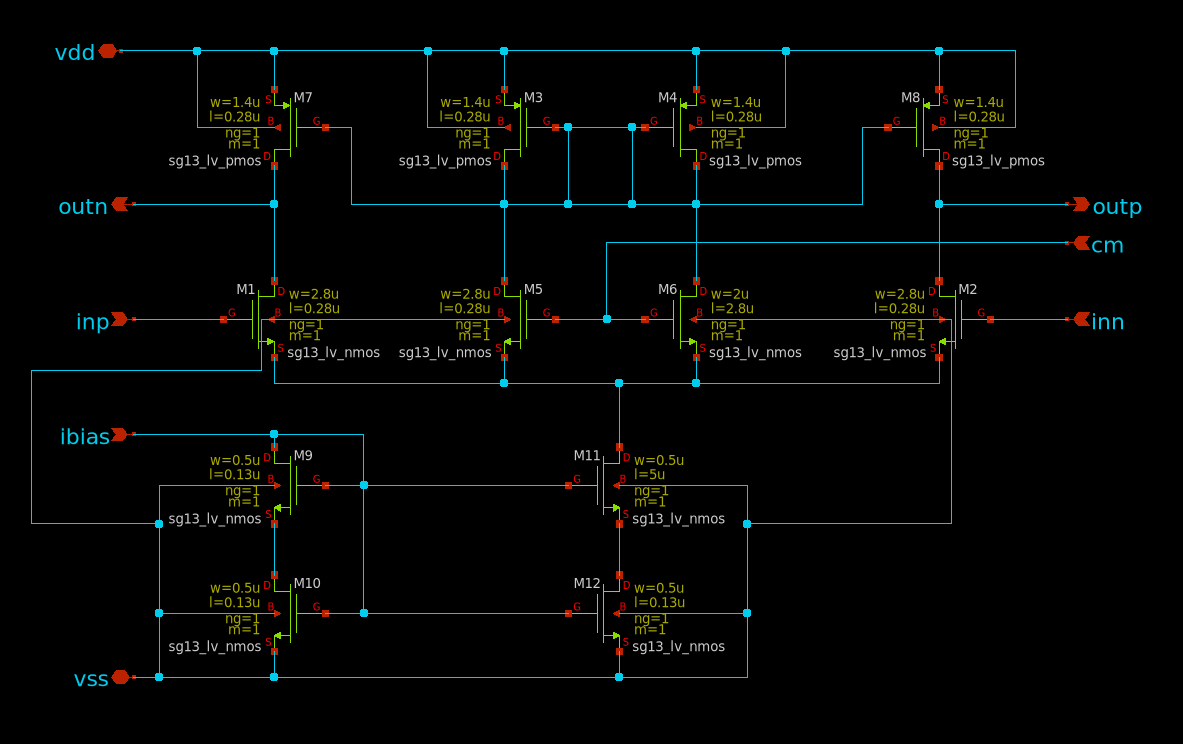
\includegraphics[keepaspectratio]{images/real-ota_gm_100u.png}}

}

\caption{\label{fig-Gm-100u-OTA}Xschem schematic of the sized
high-performance OTA.}

\end{figure}%

\subsection{Component Sizing and Filter
Design}\label{component-sizing-and-filter-design}

Despite the OTA's lower-than-desired gain, we proceeded to design the
filter's passive network. The chosen topology is a Gm-C biquadratic
filter, a versatile and tunable second-order architecture that uses
integrators made from transconductors and capacitors.

\begin{figure}

\centering{

\pandocbounded{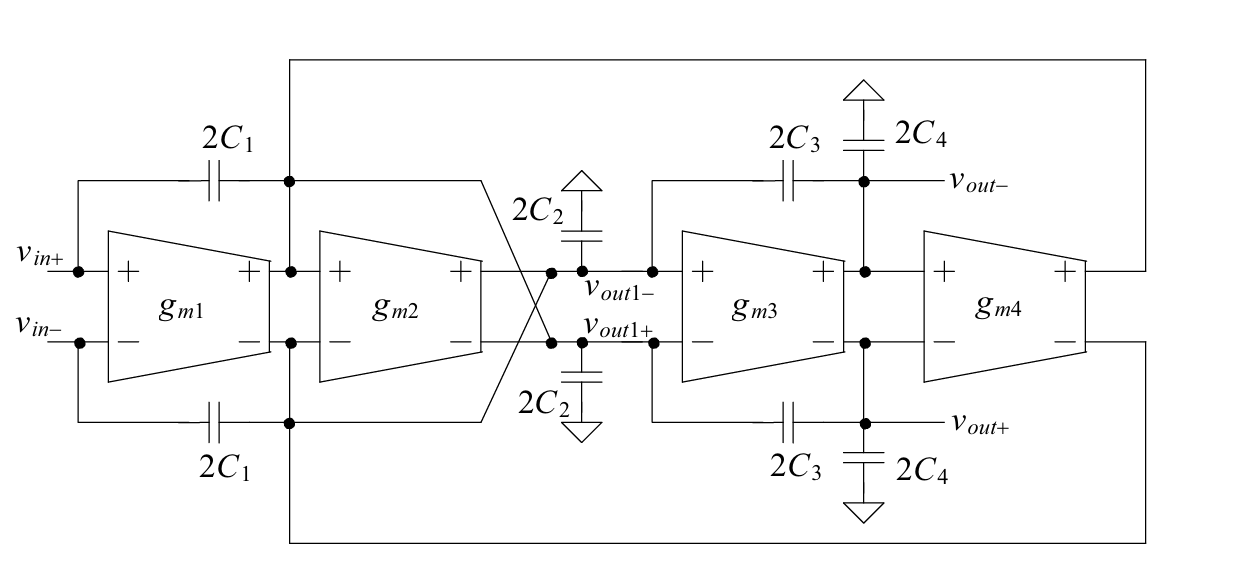
\includegraphics[keepaspectratio]{images/biquad-filter-ota-baker-book.png}}

}

\caption{\label{fig-Final-Filter-Topology}Schematic of the Gm-C Biquad
Filter Topology}

\end{figure}%

This Gm-C biquad structure is essentially a cascade of two integrator
blocks with feedback. The first stage (built around gm1, gm2, and
associated capacitors) and the second stage (built around gm3, gm4, and
capacitors) are interconnected. The feedback from the final output back
to the input creates the second-order response necessary for achieving
high Q-factors. A primary advantage of this topology is its
\textbf{electronic tunability}; the filter's center frequency (\(f_0\))
and quality factor (Q) are set by gm and C values. Since the gm can be
adjusted by changing bias currents, the filter can be tuned after
fabrication, making it ideal for integrated circuits where precise
resistor values are difficult to achieve.

\subsubsection{Design Calculations}\label{design-calculations}

The design process involves mapping the desired filter characteristics
onto the general biquad transfer function and then solving for the
specific capacitance values. Our goal is to find the values for
capacitors C1, C2, C3, and C4 to create a low-pass filter with the
following specifications: * \textbf{Center/Cutoff Frequency (\(f_0\))}:
1 kHz * \textbf{Quality Factor (Q)}: 10 * \textbf{Transconductance
(\(g_m\))}: 100 µS for gm1, gm2, gm3, and gm4.

\paragraph{Step 1: Start with the General Biquad Transfer
Function}\label{step-1-start-with-the-general-biquad-transfer-function}

The design begins with the general transfer function for the biquad
topology, which describes how the filter responds to any frequency
\texttt{s}. The numerator of the function defines the filter's zeroes
(frequencies it blocks), and the denominator defines its poles (the
natural resonant frequencies that shape the response, like \(f_0\) and
Q). The general transfer function is given by:
\[ \frac{V_{out}}{V_{in}} = \frac{s^2(G_1 G_3 G_4 G_6) + s(G_1 G_3 G_4 + G_1 G_4 G_6) + G_1 G_4}{s^2 + s(G_1 G_2 + G_1 G_4 G_5 G_6) + G_1 G_4 G_5} \]

\paragraph{Step 2: Simplify for a Low-Pass
Filter}\label{step-2-simplify-for-a-low-pass-filter}

An ideal second-order low-pass filter should only have a constant term
in the numerator, representing the DC gain.
\[ H(s)_{LP} = \frac{\text{DC Gain}}{s^2 + s\frac{\omega_0}{Q} + \omega_0^2} \]
To make our general equation match this ideal form, we must eliminate
the \texttt{s} and \texttt{s²} terms from the numerator. The simplest
way to make the coefficients of both terms zero is to set \(G_3 = 0\)
and \(G_6 = 0\). Physically, this corresponds to removing capacitors
\(C_1\) and \(C_3\), as their definitions are \(G_3 = C_1 / g_{m1}\) and
\(G_6 = C_3 / g_{m3}\).

\paragraph{Step 3: Establish the Final Design
Equations}\label{step-3-establish-the-final-design-equations}

With \(G_3=0\) and \(G_6=0\), we can equate the denominators of our
simplified transfer function and the ideal low-pass filter. This
provides our final design equations: * \textbf{Design Equation A
(\(f_0\))}: \((2\pi f_0)^2 = G_1 G_4 G_5\) * \textbf{Design Equation B
(Q)}: \(\frac{2\pi f_0}{Q} = G_1 G_2\)

\paragraph{Step 4: Calculate Capacitor
C₂}\label{step-4-calculate-capacitor-cux2082}

We start with Design Equation B. First, we substitute the component
definitions from the topology (\(G_1 = g_{m1} / C_2\) and
\(G_2 = g_{m2} / g_{m1}\)):
\[ \frac{2\pi f_0}{Q} = \left(\frac{g_{m1}}{C_2}\right) \left(\frac{g_{m2}}{g_{m1}}\right) \]
The \(g_{m1}\) terms cancel, simplifying the equation significantly:
\[ \frac{2\pi f_0}{Q} = \frac{g_{m2}}{C_2} \] Now, we rearrange to solve
for \(C_2\) and insert the specified values:
\[ C_2 = \frac{g_{m2} \times Q}{2\pi f_0} = \frac{(100 \times 10^{-6} \text{ S}) \times 10}{2 \pi \times 1000 \text{ Hz}} = \frac{0.001}{6283.2} = 1.5915 \times 10^{-7} \text{ F} \]
\[ C_2 = 159.2 \text{ nF} \]

\paragraph{Step 5: Calculate Capacitor
C₄}\label{step-5-calculate-capacitor-cux2084}

Next, we use Design Equation A. We substitute the definitions for
\(G_1\), \(G_4\), and \(G_5\):
\[ (2\pi f_0)^2 = \left(\frac{g_{m1}}{C_2}\right) \left(\frac{g_{m3}}{C_4}\right) \left(\frac{g_{m4}}{g_{m3}}\right) \]
The \(g_{m3}\) terms cancel out:
\[ (2\pi f_0)^2 = \left(\frac{g_{m1}}{C_2}\right) \left(\frac{g_{m4}}{C_4}\right) \]
From the previous step, we know that
\(\frac{g_{m1}}{C_2} = \frac{2\pi f_0}{Q}\) (since \(g_{m1}=g_{m2}\)).
Substituting this provides a more elegant path to the solution:
\[ (2\pi f_0)^2 = \left(\frac{2\pi f_0}{Q}\right) \left(\frac{g_{m4}}{C_4}\right) \]
Dividing both sides by \(2\pi f_0\) and rearranging for \(C_4\):
\[ 2\pi f_0 \times Q = \frac{g_{m4}}{C_4} \implies C_4 = \frac{g_{m4}}{2\pi f_0 \times Q} \]
Finally, we insert the values:
\[ C_4 = \frac{100 \times 10^{-6} \text{ S}}{(6283.2 \text{ rad/s}) \times 10} = \frac{100 \times 10^{-6}}{62832} = 1.5915 \times 10^{-9} \text{ F} \]
\[ C_4 = 1.59 \text{ nF} \]

\paragraph{Final Design Summary}\label{final-design-summary}

To implement the low-pass filter, the following component values are
required: \textbar{} Component \textbar{} Value \textbar{} Purpose
\textbar{}
\textbar-----------------\textbar----------------\textbar-----------------------------------------\textbar{}
\textbar{} \(g_{m1,2,3,4}\) \textbar{} 100 µS \textbar{} Sets filter
gain and characteristics \textbar{} \textbar{} \(C_1\) \textbar{} 0 F
(removed) \textbar{} Simplifies filter to low-pass response \textbar{}
\textbar{} \(C_2\) \textbar{} 159.2 nF \textbar{} Sets the Q-factor
\textbar{} \textbar{} \(C_3\) \textbar{} 0 F (removed) \textbar{}
Simplifies filter to low-pass response \textbar{} \textbar{} \(C_4\)
\textbar{} 1.59 nF \textbar{} Sets the center frequency, \(f_0\)
\textbar{}

\begin{tcolorbox}[enhanced jigsaw, bottomrule=.15mm, leftrule=.75mm, breakable, coltitle=black, left=2mm, titlerule=0mm, opacityback=0, rightrule=.15mm, toprule=.15mm, arc=.35mm, colback=white, colbacktitle=quarto-callout-note-color!10!white, bottomtitle=1mm, colframe=quarto-callout-note-color-frame, toptitle=1mm, title=\textcolor{quarto-callout-note-color}{\faInfo}\hspace{0.5em}{A Note on Practicality and Component Values}, opacitybacktitle=0.6]

A critical review of these final component values reveals a significant
practical challenge. The calculated capacitors, particularly
\(C_2 = 159.2 \text{ nF}\), are enormously large for on-chip
implementation.

For context, at a typical Metal-Insulator-Metal (MIM) capacitor density
for the SG13G2 process (around 1-2 fF/µm²), a 159.2 nF capacitor would
occupy an area of roughly 80-160 mm². This is prohibitively large, often
exceeding the area of an entire die, and thus is completely impractical
for a monolithic integrated circuit.

This issue arises directly from the design specifications: a very low
target frequency (\(f_0 = 1 \text{ kHz}\)) combined with a moderately
high transconductance (\(g_m = 100 \text{ µS}\)). For a production-ready
design, a mandatory next step would be to re-evaluate these
specifications. The most common approach would be to drastically reduce
the OTA's transconductance (e.g., to 1 µS or less), which would
proportionally decrease the required capacitance to a manageable level
(e.g., \(C_2 \approx 1.6 \text{ nF}\)).

For the purpose of this academic exercise, we will proceed with the
calculated values to demonstrate the correctness of the design
methodology and to verify the filter's transfer function in simulation.

\end{tcolorbox}

\subsection{Final Implementation and
Verification}\label{final-implementation-and-verification}

The final Gm-C biquad filter was assembled in Xschem using the newly
designed OTAs and calculated capacitors.

\begin{figure}

\centering{

\pandocbounded{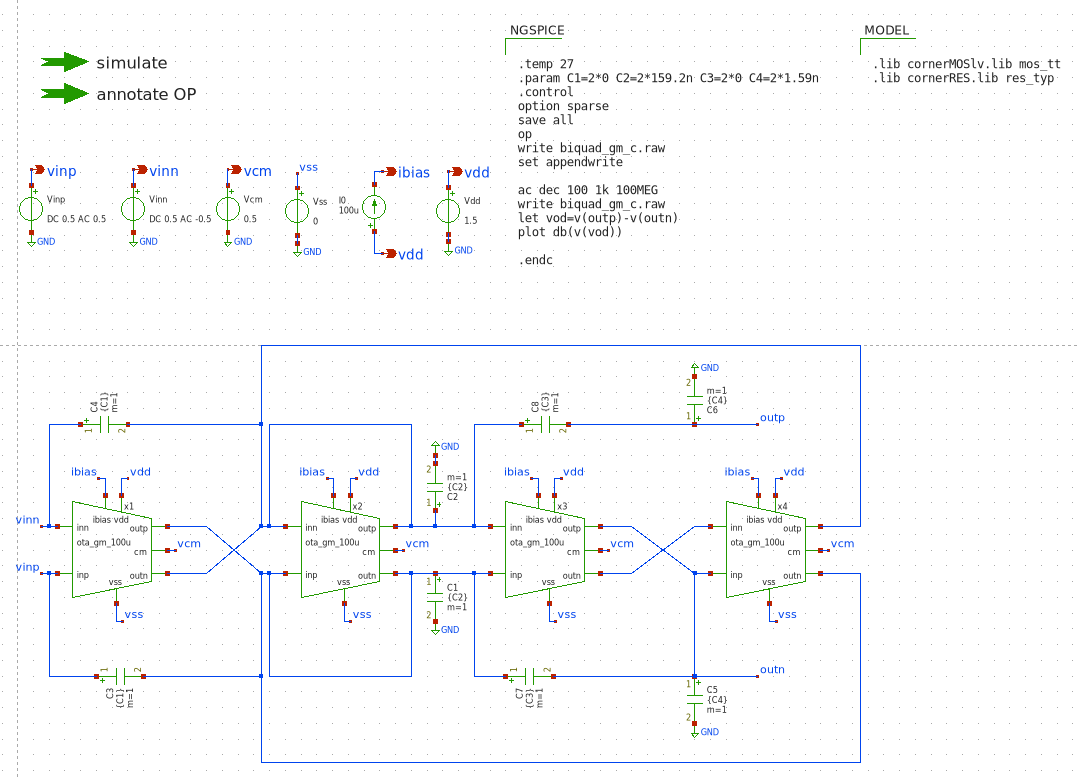
\includegraphics[keepaspectratio]{images/real-biquad_gm_c.png}}

}

\caption{\label{fig-Final-Biquad}Final Xschem schematic of the Gm-C
biquad filter.}

\end{figure}%

AC analysis was performed, with the expected output being a low-pass
response with a sharp resonant peak at 1 kHz due to the high Q-factor,
followed by a -40 dB/decade roll-off.

\begin{figure}

\centering{

\pandocbounded{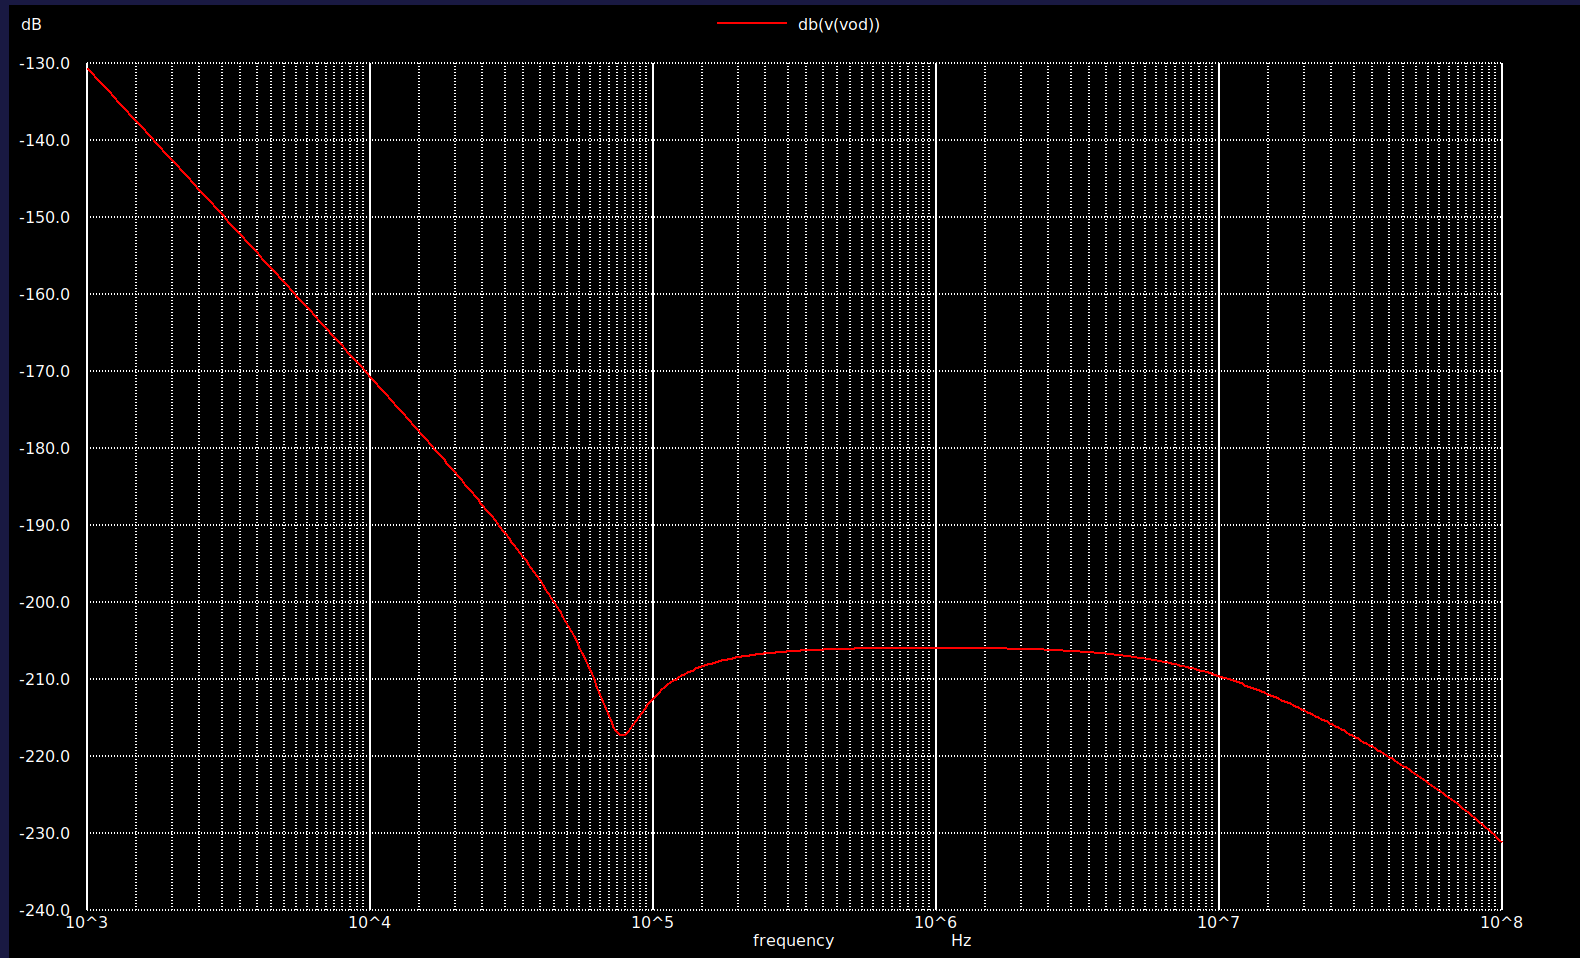
\includegraphics[keepaspectratio]{images/real-biquad_gm_c-output.png}}

}

\caption{\label{fig-Final-Bode}Simulated Bode plot of the final low-pass
filter.}

\end{figure}%

The simulation confirms the filter is operating as designed. The success
of the final filter, even with a sub-optimal OTA, demonstrates the
robustness of the Gm-C biquad topology. It suggests that while higher
OTA gain would improve performance (e.g., Q-factor accuracy), the
fundamental design is sound.

\chapter{Conclusion}\label{conclusion-1}

\chapter*{References}\label{references}
\addcontentsline{toc}{chapter}{References}

\phantomsection\label{refs}




\end{document}
